%\chapter{Grafeno}

El grafeno es un nanomaterial 2-dimensional formado por átomos de carbono en hibridización sp2 \footnote{Véase anexo \ref{sec:hibridacion_sp2}}, dispuestos en una estructura de panal de abeja, esta estructura no es una red de Bravais pero puede ser descrita por una red hexagonal con una base de dos átomos de carbono (ver figura \ref{fig_graphene_lattice}). 

\begin{figure}
	\centering
	\fbox{
		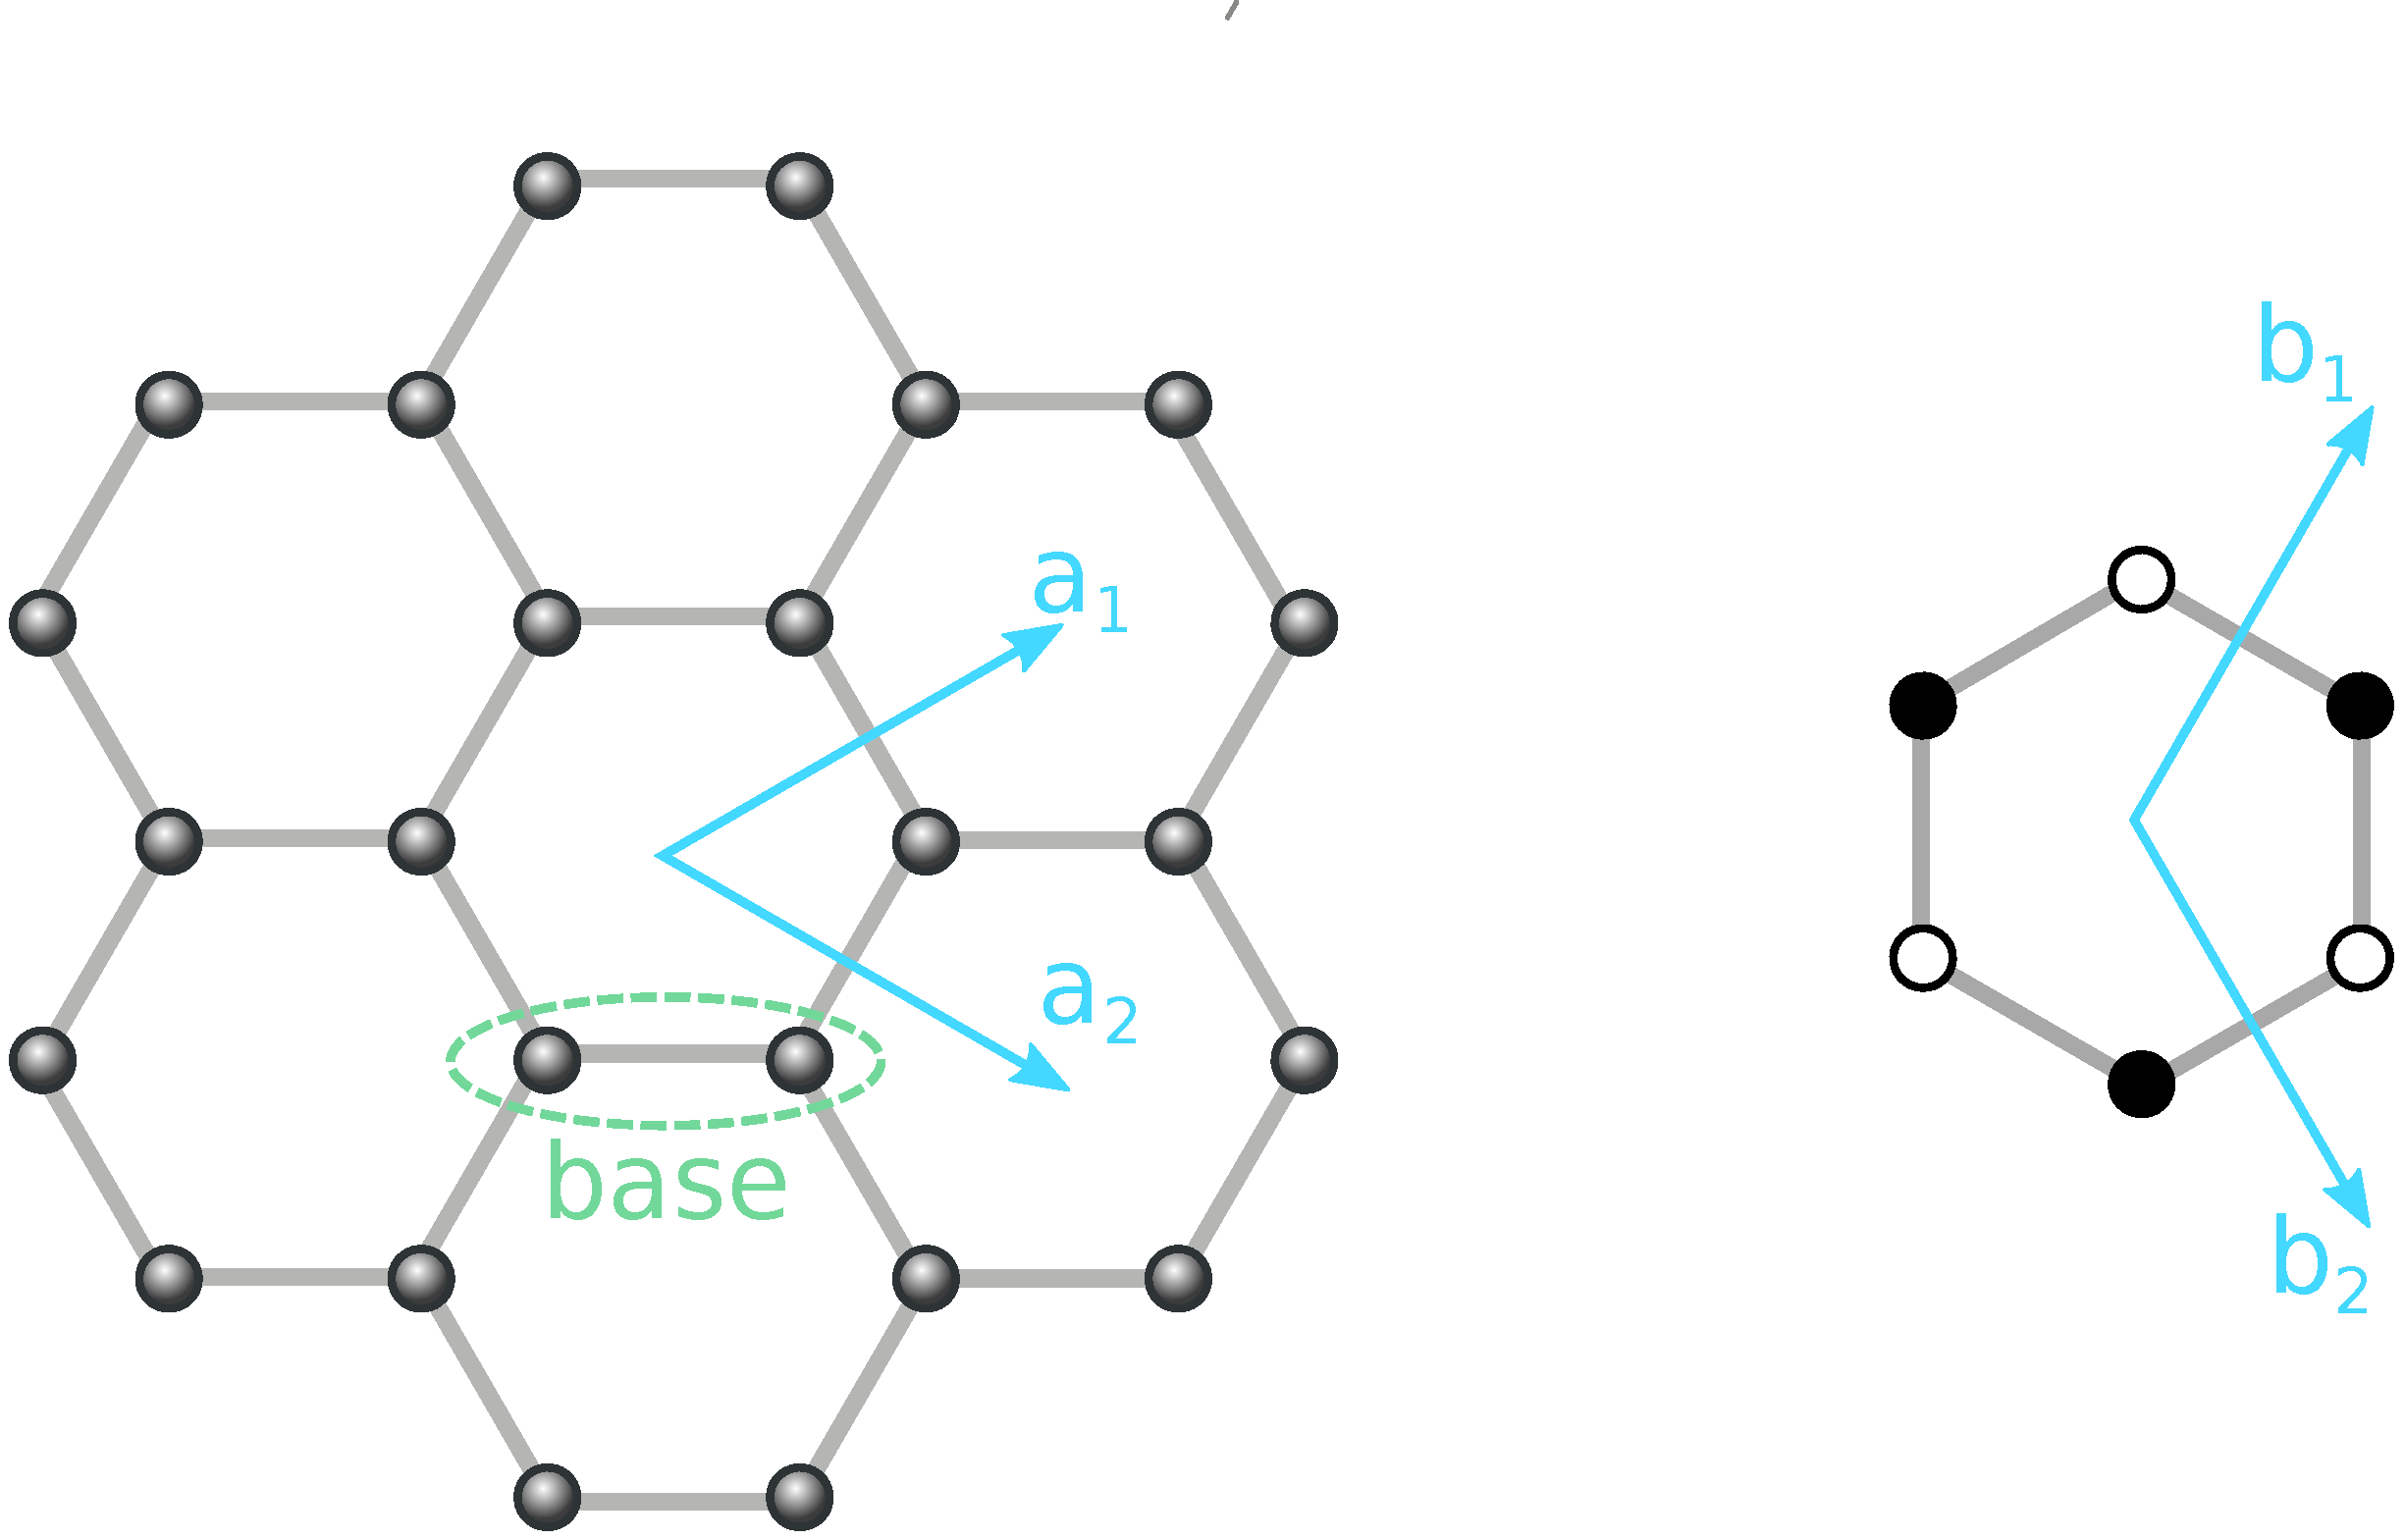
\includegraphics[width=0.75\textwidth]{graphene_lattice.pdf}
		}
	\caption[Estructura del grafeno]{Izquierda: Red de grafeno en espacio real. Derecha: Red en espacio recíproco.}
	\label{fig_graphene_lattice}
\end{figure}

El primero en tratar con este material fue probablemente Brodie \citep{Brodie1859} que al exponer grafito a ácidos fuertes, creyó descubrir una nueva forma de carbono a la que llamó grafón, ahora se sabe que lo que observó fue óxido de grafeno, esto es, láminas de grafeno recubiertas por grupos epóxi e hidroxilo \citep{Geim2012}. Wallace, dio con los primeros estudios teóricos sobre el grafeno al estudiar la estructura de bandas del grafito, pero como una simplificación de tal estructura \citep{Wallace1947}. Fue Boehm quien le dio el nombre al crear la nomenclatura y terminología para compuestos de grafito intercalado \citep{Boehm1986}. No fue hasta 2004 que Novoselov, Geim y otros, lograron aislar grafeno por medios mecánicos \citep{Novoselov2004}, por lo que les fue otorgado el Premio Nobel de Física en el año 2010.

El grafeno presenta propiedades extraordinarias, como ha sido demostrado en numerosos experimentos: movilidad electrónica de 200.000 $\mathrm{cm^2 V^{-1} s^{-1} }$ \citep{Bolotin2008}, tensión de ruptura de 130 GPa, y módulo de Young de 1.0 TPa \citep{Lee2008}, conductividad térmica entre 600 a 5000 $\mathrm{W\, mK^{-1}}$ \citep{Balandin2011}, opacidad de 2,3\% y reflectacia menor al 0,1\% \citep{Nair2008}, impermeable totalmente a gases estándar \citep{Bunch2008} y resistir densidades de corriente muy grandes de hasta $\mathrm{10^8 A\, cm^{-2}}$ sin sufrir daños  \citep{Moser2007}. Tiene un área superficial específica calculada de 2630 $\mathrm{m^2 g^{-1}}$ \citep{Peigney2001}. Es importante notar que estos resultados se han obtenido en muestras muy puras de grafeno exfoliado mecánicamente \citep{Novoselov2004} y están lejos de ser replicables a gran escala. Otros métodos de sintesis incluyen: exfoliación térmica y en fase líquida del grafito\citep{Blake2008}, deposición química de vapor (CVD) en sustratos de cobre, sublimación de los átomos de silicio en carburo de silicio\citep{DeHeer2011a},   Es por esto que, se hace necesario encontrar métodos de síntesis de producción de grafeno con propiedades similares a las citadas anteriormente bajo procesos de alta escalabilidad industrial \citep{Novoselov2012}.

\subsection{Óxido de grafeno (GO)}
Una de las formas de obtener grandes cantidades de grafeno es mediante la llamada ruta de "óxido de grafeno" (figura \ref{fig:graphiteToRGO}), en la cual el grafeno es decorado densamente por grupos epóxi, hidroxilo, y carboxilo \citep{Dreyer2010}. Estos grupos ricos en oxígeno presentes en la red del grafeno se presentan como defectos en la red cristalina, cambiando sus propiedades drásticamente. Varias estructuras han sido propuestas para el óxido de grafeno (figura \ref{fig:GO_structure}).
El óxido de grafeno es sintetizado a partir de grafito natural, exponiéndolo a agentes oxidantes fuertes, una sustancia capaz de remover electrones y entregar átomos electronegativos. Esto introduce grupos funcionales ricos en oxígeno entre los planos de grafeno del grafito, aumentado la distancia interplanar, y disminuyendo la fuerza de atracción entre monocapas, facilitando la separación de capas de grafeno (ahora óxido de grafeno). La mayoría de los métodos de síntesis de óxido de grafeno se basan en alguno de los tres siguientes: método de Brodie \citep{Brodie1859}, método de Staudenmaier \citep{Staudenmaier1898}, o método de Hummers \citep{Hummers1958}. En breve, en el método de Brodie, clorato de potasio (\ce{KClO_3}) se agrega a una mezcla de grafito y ácido nítrico (\ce{HNO_3}), produciendo óxido de grafito, Brodie empleó este método en busqueda de la fórmnula molecular del grafito. Tiempo después, Staudenmaier mejoró el procedimiento agregando el clorato de potasio gradualmente y adicionando ácido sulfúrico (\ce{H_2SO_4}). Casi 60 años después, Hummers y Offeman desarrollaron un método alternativo utilizando permanganato de potasio (\ce{KMnO_4}) y ácido sulfúrico, alcanzando niveles de oxidación parecidos a los métodos de Brodie y Staudenmaier.

\begin{figure}
	\centering
	\fbox{
		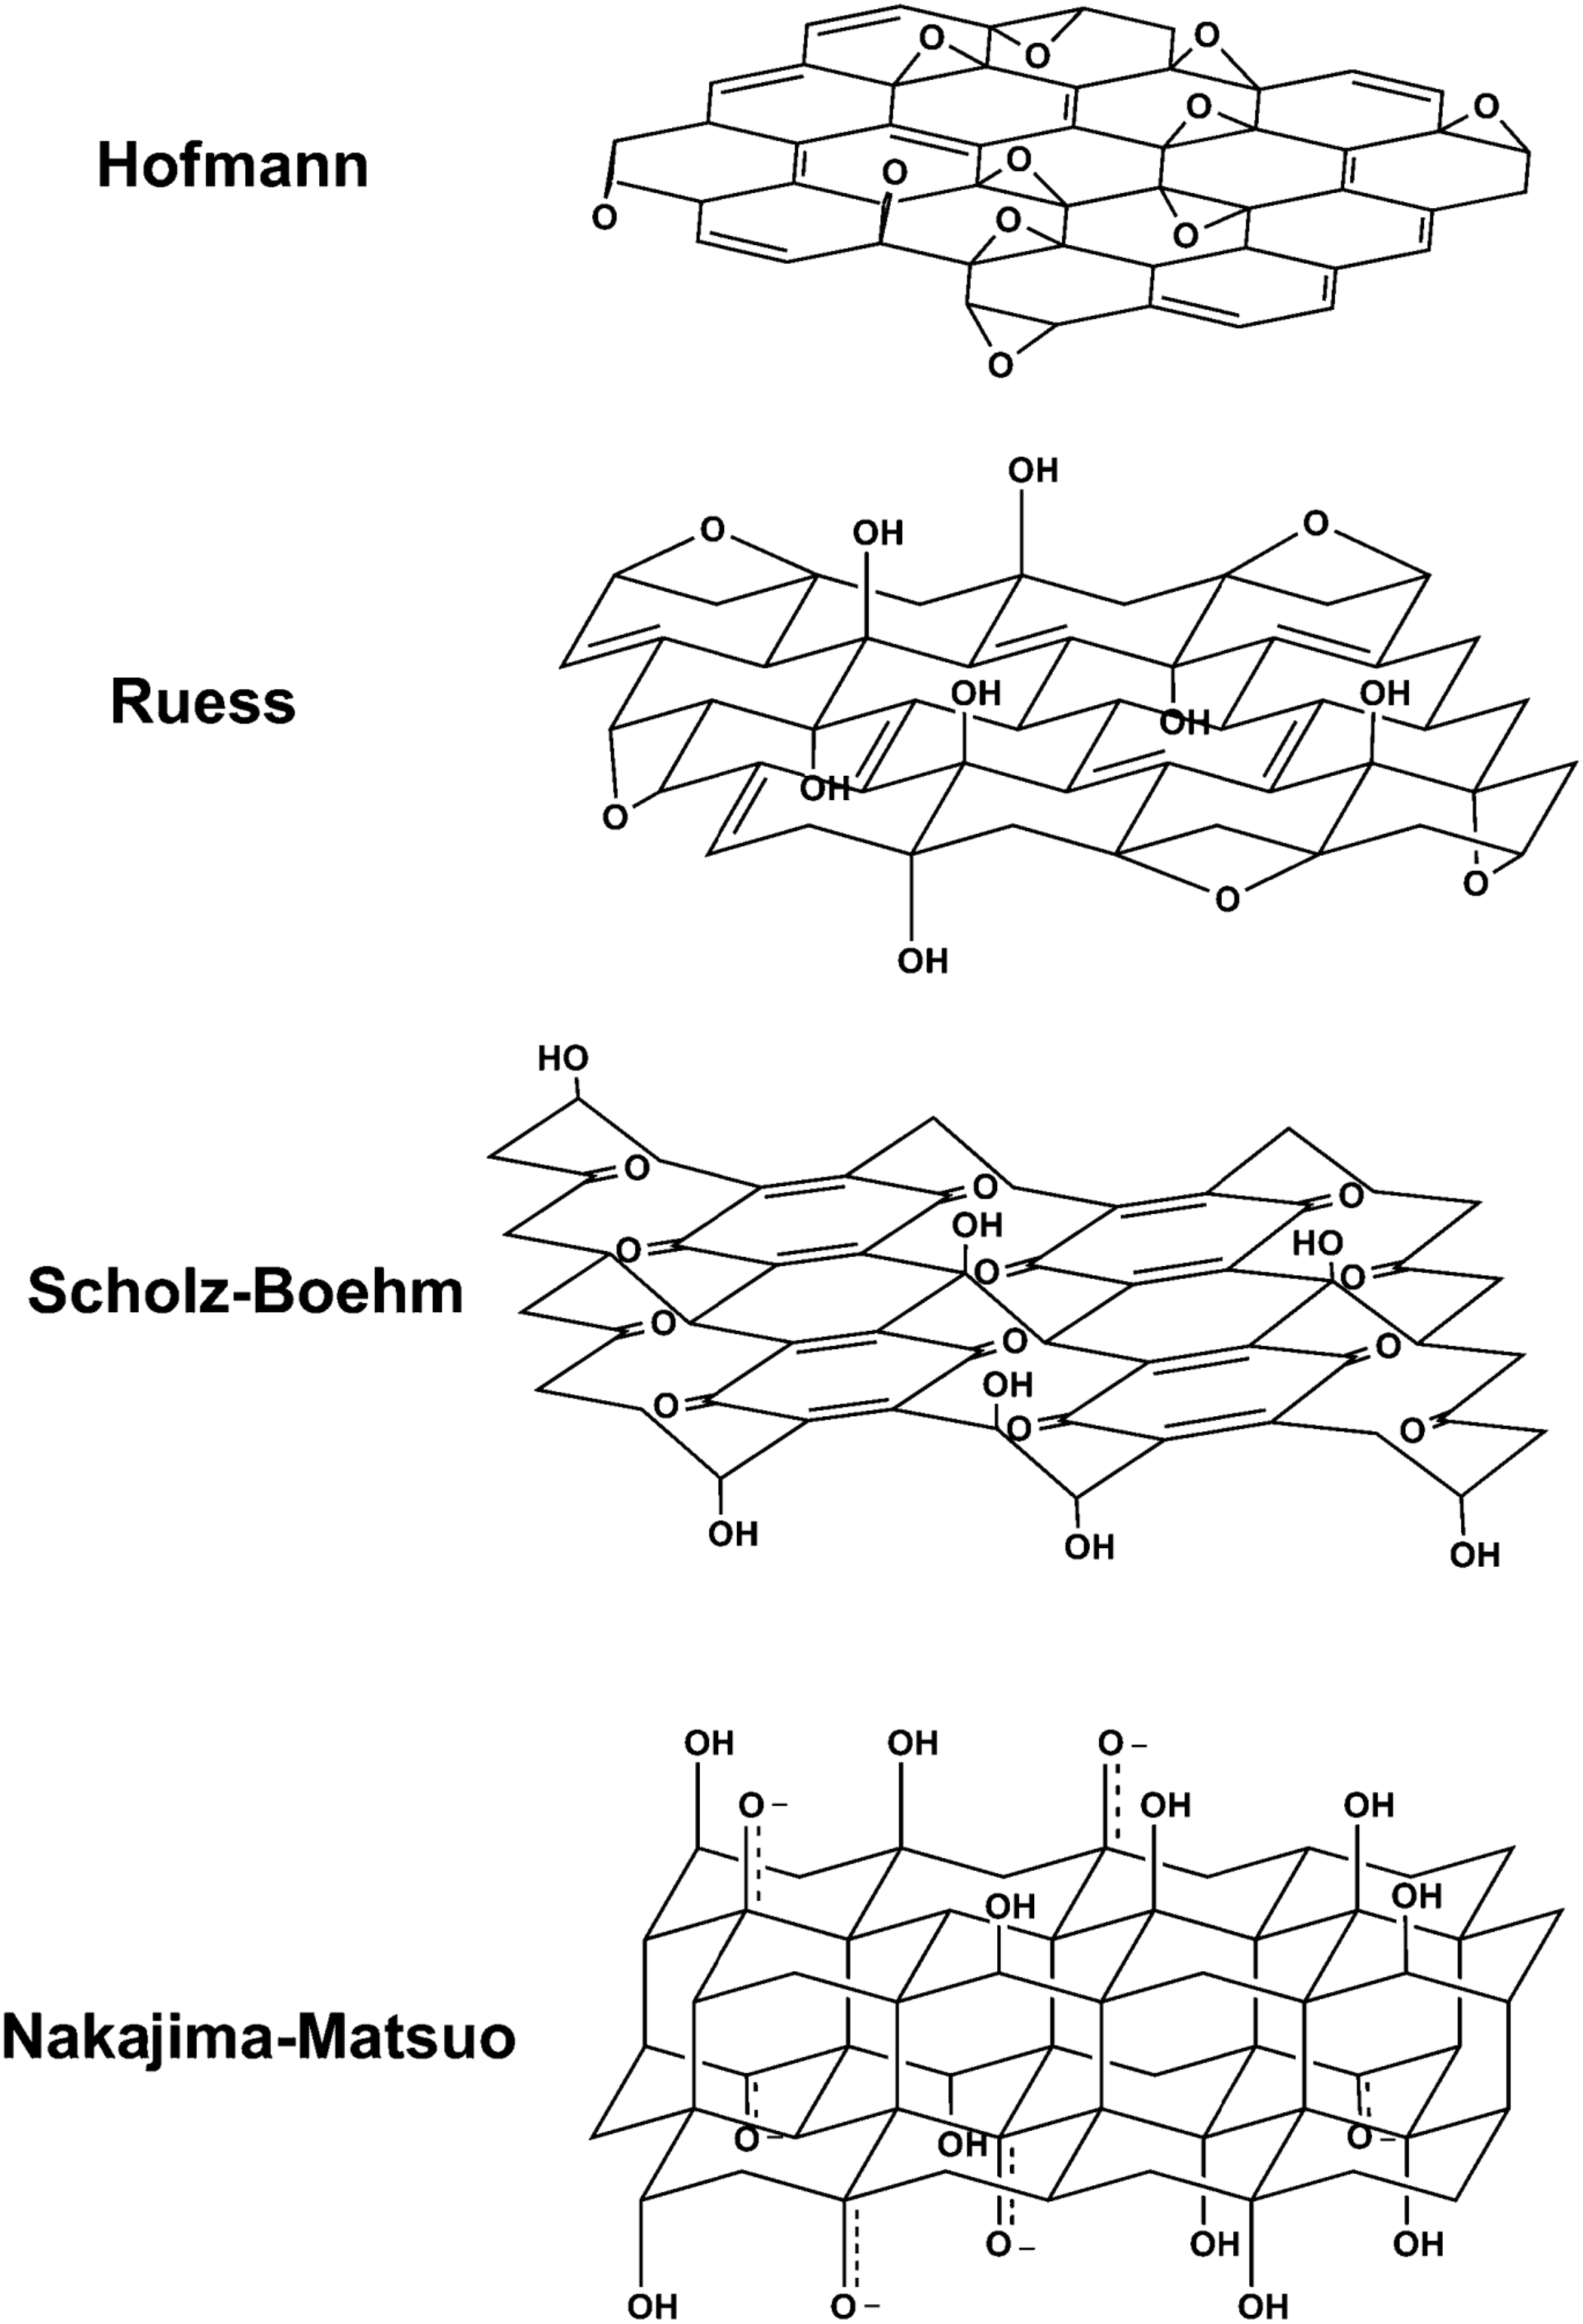
\includegraphics[width=0.5\textwidth]{GO_structure.pdf}
	}
	\caption[Estructura de óxido de grafeno]{Estructuras propuestas para el óxido de grafeno \citep{Dreyer2010}.}
	\label{fig:GO_structure}
\end{figure}


\subsection{Reducción del óxido de grafeno}
Los grupos funcionales presentes en el óxido de grafeno pueden ser removidos para volver a la estructura del grafeno como tal.
Existen muchas formas de reducir el óxido de grafeno, por medios químicos, térmicos, o electroquímicos. El método de reducción química cosiste en exponer al óxido de grafeno a un agente reductor, como es el caso de la hidrazina , o el ácido ascórbico \citep{Fernandez-Merino2010}, cuyos poderes de reducción son bien conocidos y ampliamente difundidos en la literatura científica \citep{Chua2015}. Por otro lado, la reducción térmica contempla la exposición del óxido de grafeno a altas temperaturas, provocando que los grupos que contienen oxígeno descompongan en gases como \ce{CO_2}, además, si el óxido de grafeno no está completamente exfoliado, la presión de los gases generados puede separar las capas \citep{Pei2012}. Esta reducción puede llevarse a cabo en un horno convencional, por microondas en un horno microondas comercial \citep{Zhu2010a}, por láser \citep{El-Kady2013}, por plasma \citep{Lee2012}, o por luz solar concentrada \citep{Mohandoss2017}. En el caso del proceso electroquímico, la reducción se realiza en presencia de un solvente, donde el óxido de grafeno puede estar disperso en el solvente \citep{Liu2011}, depositado en un electrodo \citep{Harima2011, Toh2014}, o bien ser el cátodo por sí mismo \citep{Feng2016}. La ventaja del método electroquímico, es la facilidad de realizar electrodeposición del óxido reducido de grafeno en el ánodo y la combinación con otros nanomateriales, como por ejemplo, una síntesis \emph{in-situ} de nanocompuestos \citep{Liu2011, Xie2014}.


\begin{figure}
	\centering
	\fbox{
		\includegraphics[width=\textwidth]{graphiteToRGO.pdf}
	}
	\caption{Síntesis de grafeno a través de la ruta del óxido de grafeno.}
	\label{fig:graphiteToRGO}
\end{figure}

\subsection{Aplicaciones}
El óxido reducido de grafeno encuentra su lugar en aplicaciones que requieran gran cantidad de material o gran área superficial específica, como en baterías \citep{Li2014}, supercondensadores \citep{Stoller2008} o celdas solares \citep{Roy-mayhew2014}, o donde sea necesario funcionalizar la superficie del grafeno como sucede en distintos tipos de sensores \citep{Schedin2007, Haick2013}.

